\documentclass[a4paper, 12pt]{article}

\usepackage{listings}
\usepackage{color}
\usepackage[frenchb]{babel}
\usepackage[utf8]{inputenc}
\usepackage[T1]{fontenc}
\usepackage{lmodern}
\usepackage{graphicx}
% Numbers and units
\usepackage[squaren, Gray]{SIunits}
\usepackage{sistyle}
\usepackage[autolanguage]{numprint}
\usepackage{fullpage}

\usepackage{multirow}
\usepackage{xparse}
\usepackage{tikz}
\usepackage{enumitem}
\setlength{\parskip}{1em}
\usetikzlibrary{arrows, decorations.markings}

\newcommand\si[2]{\numprint[#2]{#1}}
\newcommand\np[1]{\numprint{#1}}

\newcommand\figref[1]{figure~\ref{fig:#1}}

\NewDocumentEnvironment{myfig}{mm}
{\begin{figure}[!ht]\centering}
{\caption{#2}\label{#1}\end{figure}}

\usepackage[Conny]{fncychap}

\usepackage{enumerate}

\lstset{ %
  backgroundcolor=\color{white},   % choose the background color; you must add \usepackage{color} or \usepackage{xcolor}
  basicstyle=\footnotesize,        % the size of the fonts that are used for the code
  breakatwhitespace=false,         % sets if automatic breaks should only happen at whitespace
  breaklines=true,                 % sets automatic line breaking
  captionpos=b,                    % sets the caption-position to bottom
  commentstyle=\color{mygreen},    % comment style
  deletekeywords={...},            % if you want to delete keywords from the given language
  escapeinside={\%*}{*)},          % if you want to add LaTeX within your code
  extendedchars=true,              % lets you use non-ASCII characters; for 8-bits encodings only, does not work with UTF-8
  frame=single,                    % adds a frame around the code
  keywordstyle=\color{blue},       % keyword style
  language=Java,                   % the language of the code
  morekeywords={*,...},            % if you want to add more keywords to the set
  numbers=left,                    % where to put the line-numbers; possible values are (none, left, right)
  numbersep=5pt,                   % how far the line-numbers are from the code
  numberstyle=\tiny\color{mygray}, % the style that is used for the line-numbers
  rulecolor=\color{black},         % if not set, the frame-color may be changed on line-breaks within not-black text (e.g. comments (green here))
  showspaces=false,                % show spaces everywhere adding particular underscores; it overrides 'showstringspaces'
  showstringspaces=false,          % underline spaces within strings only
  showtabs=false,                  % show tabs within strings adding particular underscores
  stepnumber=1,                    % the step between two line-numbers. If it's 1, each line will be numbered
  stringstyle=\color{mymauve},     % string literal style
  tabsize=2,                       % sets default tabsize to 2 spaces
  columns=flexible,
  title=\lstname                   % show the filename of files included with \lstinputlisting; also try caption instead of title
}

\title{Formalizing Refactorings with Graph Transformation}
\author{Paulus Alois}

\begin{document}

\maketitle

\tableofcontents

\newpage

\section{Introduction}

Qu'est ce que le refactoring ? 

Le refactoring permet de changer la structure d'un programme en vue de l'améliorer tout en préservant son comportement. 

Il consiste à déplacer des méthodes, renomer des variables, crée des fonctions ect et est généralement appliqué sur des programmes écrit en language orienté objet. 

Il peut être éffectué à la main, le programmeur va analyser le code et identifier des parties de code à modifier. Ensuite il va apporter les modifications necessaires au programme.
Cette technique est assez lente et surtout peu sure, en effet le programmeur peu faire des erreurs et introduire des bugs.

Pour pallier à ça, des outils de refactoring sont disponibles et permettent d'automatiser les actions comme le renomage d'une variable, le déplacement d'un fonction ect. Tout en garantissant une certaine sécurité.

Ces outils ne sont malheureusement pas parfait, ils sont pour la plupart spécialisé dans un seul language de programmation et ne garantisent pas à 100 pourcent la préservation du comportement du programme.

Cet article va présenter une approche permettant de crée un outil générique et mathématiquement vérifiable. La structure des programmes sera représentée au moyen de graph et le refactoring equivalera à des transformations de ces graphs.

L'avantage des transformations de graph est qu'elles sont vérifiables mathématiquement, ce qui permettra de garentir la conservation de certaines propriétés des programmes.

Ainsi nous auront la possibilité de refactorer de manière automatisée sur multiple language de programmation en étant certain de conserver les fonctionnalités de notre programme.

\newpage 

\section{Représentation en graph}
Pour représenter la structure d'un programme orienté objet et les règles de refactoring nous aurons besoin de plusieurs type de graph.

\begin{itemize}[label=\textbullet]
\item Les graphs de type
\item Les graphs de programme
\item Les graphs d'expression
\end{itemize}

En vue de pouvoir s'integrer au mieux dans les logiciels de refactoring, la représentation en graph s'approchera le plus possible d'un arbre de syntaxe abstrait augmenté de lien.

Il est également important que le model reste conci pour facilité sa compréhension. De ce faite nous incluerons uniquement les choses requisent pour prouver les propriétés du refactoring.

\subsection{Les différents type de graph}

\subsection{Le graph de type}

Le graph de type sert à spécifier les différentes contraintes qu'un graph de programme devra respecter. Un graph de programme devrat respecter toutes ces contraintes ou bien être condidéré comme un programme syntaxiquement incorrecte. De manière plus concraite, ce programme ne compilera pas.

Il est donc indispensable d'établir un graph de type pour prouver que le refactoring produit des programmes valide.

Malheureusement, le graph de type ne suffit pas à représenter toutes les contraintes voir figure~\ref{contraintes}, il faut également y joindre un ensemble de sous graph interdit.

De plus cet ensemble de graph interdit peut être infini. Par exemple contenir plusieurs variables avec le même nom consiste a interdir tous les graphs avec deux ou plus variable de même nom.

Pour régler ce problème nous auront besoin des graphs d'expression expliqué ci dessous.\label{subsec:graphExpression}


\begin{myfig}{contraintes}{Exemple de contrainte non représentable}
\begin{enumerate}
 \scriptsize \item une classe ne peut pas contenir plusieurs variables avec le même nom
 \scriptsize \item une classe ne peut pas contenir plusieurs méthode avec la même signature
 \scriptsize \item une expression contenue dans une méthode ne peut pas accéder à des variables contenues dans les descendants de la classe
 \scriptsize \item une expression contenue dans une méthode ne peut pas accéder à un paramètre appartenent à une autre méthode.
\end{enumerate}
\end{myfig}

\subsubsection{Définition}
Un graph de type est un graph labellé contenant un ensemble de noeuds typé et d'arrêtes typée. G étant un graph et TG un graph typé. G est typé par rapport à TG si il existe une projection
de G dans TG conservant les sources, les targets et les labèles. Pour les labèles on prend en compte uniquement le label.

\subsubsection{Les differents type de node}

  \begin{tabular}{ | l | l | l | p{5cm} |}
    \hline
    type & description  \\ \hline
    C & Class   \\ \hline
    M & Signature de méthode   \\ \hline
    MD &  Définition d'une méthode   \\ \hline
    V &  Variable   \\ \hline
    VD &  Définition d'une variable \\ \hline
    P & Paramètre \\ \hline
    E &  Expression contenue dans une définition de méthode \\ \hline
    \end{tabular}

\subsubsection{Les différents type d'arrêtes}
  \begin{tabular}{ | l | l |  l |}
    \hline type & application & description  \\ \hline
    l : & M -> MD & \\ & V -> VD & lookup d'une variable ou d'une méthode à sa définition \\ \hline 
    i : & C -> C &  héritage d'une classe à une autre de méthode    \\ \hline
    m : & VD -> C & \\ & MD -> C & appartenance d'un variable ou d'une méthode à une classe  \\ \hline
    t : & V -> C  & \\ &  M -> C & type d'une variable ou type de retour    \\ \hline
    p : & MD -> P  & \\ &  P -> C & définition d'un paramètre ou de son type     \\ \hline
    e : & E -> M & expression contenue dans une définition de méthode ou \\ & &  dans une expréssion    \\ \hline
    a : & E -> {V|P} & accèss à une variable ou à un paramètre    \\ \hline
    u : & E -> {V|P} & mise à jour d'une variable ou d'un paramètre    \\ \hline
   \end{tabular}

\begin{myfig}{typeGraph}{Graph de type}
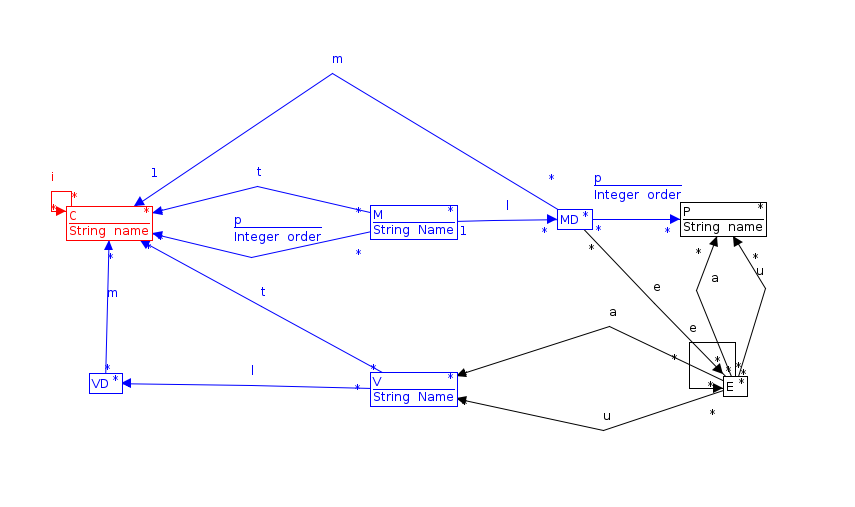
\includegraphics[width=\textwidth]{typeGraph.png}
\end{myfig}

La figure~\ref{typeGraph} est un exemple de graph de type, on peut observer toutes les relations possible entre les type de noeuds et d'arrêtes.
Et grâce au tableau ci dessous vous pouvez interpreter ce graphique.

Voici quelques exemples:
\begin{enumerate}
Les noeuds C peut ainsi hériter d'un autre noeud C.
Les noeuds MD contiendra des noeuds E et appartiendra à un noeud C
Les noeuds V auront comme type un noeud C
Les noeuds E pourront mettre à jour ou bien accèder à un noeud V
\end{enumerate}


\subsection{Les graphs de programme} 

Graph typé et labelé représentant le code source un programme. Il est composé de noeuds typés reliés par des arrêtes typées. Ses noeuds et ses arrêtes prennent les valeurs vu dans le graph de type figure~\ref{typeGraph} et sont agrémentés d'un nom et/ou d'autres attributs. La figure~\ref{typedGraph} est un exemple de graph de programme.

\subsubsection{Definition}
G est composé d'un ensemble de noeuds labelés et d'arrêtes labelées, c'est un graph formé de triplet, ({$V_G$},{$E_G$},nlabg), ou {$V_G$} est un ensemble de noeuds, nlabg est une function de nomage de noeud et {$E_g$} est un ensemble d'arrêtes. Les arrêtes sont représentées par un triplet (noeud depart, label, noeud destination).

Dans un graph de programme les entité (classes, variables, méthodes et paramètres) sont représentés par des noeuds dont le label est une paire composée d'un nom et d'un type.

Les relations entre ces différentes entités (héritage, appelle de méthodes, appartenance) sont représentées par des arrêtes. Ces arrêtes possèdent un label pour faire la différence entre les arrêtes de même type ayant le même noeud source et le même noeud destination.

\begin{myfig}{typedGraph}{Graph de programme}
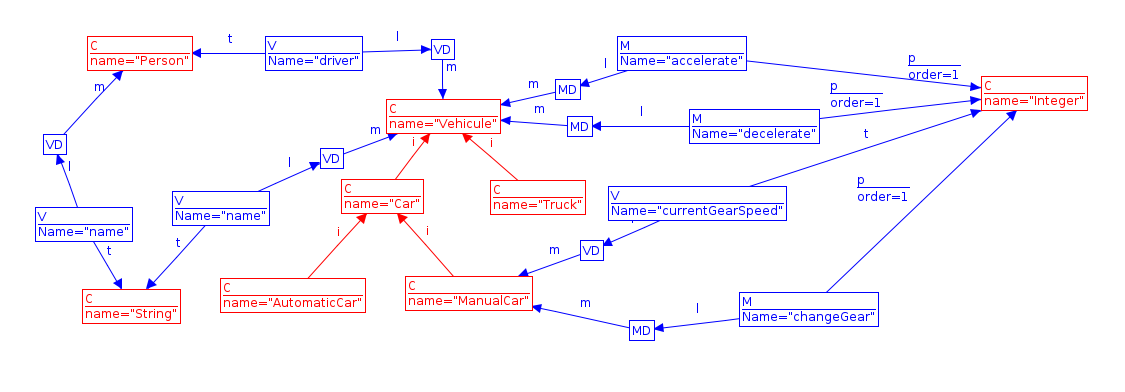
\includegraphics[width=\textwidth]{typedGraph.png}
\end{myfig}

\subsection{Les graph d'expression} 

Dans la section~\ref{subsec:graphExpression} nous avons évoqué les graphs d'expression en vue de représenter des contraintes supplémentaires. 

Ces graphs possèdent des arrêtes avec des labels pouvant être des expressions régulières. Ce qui permet de représenter un ensemble de graph à partir d'un seul, Il suffit de remplacer les expressions régulières par leurs valeurs et de créer un graph pour chacune de celle çi. Voici un exemple figure~\ref{graphExpression}

\begin{myfig}{graphExpression}{Graph d'expression}
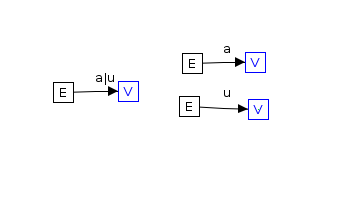
\includegraphics{graphExpression.png}
\end{myfig}

A gauche de la figure~\ref{graphExpression}, se trouve un graph avec une arrête dont le label est une expression régulières. A droite sont représenté les deux graphs possible issu du premier graph qui montre une expression méttant à jour une variable ou un expression accédant à une variable.

L'exemple reste assez simple mais vous pouvez imaginer un graph qui peut representer des centaines d'autres graphs.

\section{Cas d'étude}

Durant tout l'article, nous étudierons deux refactoring en particulier. 

\begin{enumerate}
\item PullUpMethod qui consiste à supprimer une méthode présente dans une ou plusieur classes enfant et à l'insérer dans la classe parent.
\item EncapsulateVariable qui consiste à imposer l'accès et la mise à jour d'une variable par l'intermédiaire de deux méthodes communémant appelé getter et setter.
\end{enumerate}

Les exemples seront prit sur base du programme "Transport", c'est un programme simple écrit en java permettant ces deux refactorings.

Certains exemples seront donné sous forme de graph. Dans la plupart des cas, ces graphs ont été réalisé grâce à l'outil AGG. 

Les caractèristique de AGG sont:

\begin{itemize}[label=\textbullet]
\item Représenter des structures de donnée sous forme de graph qui peuvent être typé par un graph de type.
\item Spécifier des règles sur un graph
\item Spécifier des "NAC" pour exprimé la non-existance de certaines structures lors de transformation de graph
\item Application de transformation de graph
\item Application séquentiel de transformation de graph
\end{itemize}

AGG est assez facile à prendre en main, surtout gràce aux exemples fournis. Il m'a aidé à comprendre certains concepts comme les NACs et m'a été très utile durant toute la rédaction de mon rapport.

\subsection{Programme Transport}

\begin{lstlisting}[frame=single]
public class Vehicule {
	public String name;
	public Person driver;

	public void accelerating(int amount) {

	}

	public void decelerate(int amount) {
	
	}
}

public class Truck extends Vehicule {

}

public class Person {
	public String name;
}

public class ManualCar {
	public int currentGearSpeed;
	
	public void changeGear(int number) {
	}
}

public class Car extends Vehicule {

}

public class AutomaticCar {

}
\end{lstlisting}

\newpage
\section{Refactoring}

\subsection{Preservation du comportement}
\label{subsec:preservationDuComportement}

La conservation du comportement d'un programme est une chose primordiale lors d'un refactoring. malheureusement , il n'est pas facile de définir en quoi consiste réellement cette préservation, il est même impossible de la garantir à 100 pourcent. 

Par ailleurs il sera nécessaire de trouver une définition garantissant que le programme effectuera les mêmes actions avant et après le refactoring. 

Dans cette optique, nous nous concentrerons ici sur trois proprieté.

\begin{itemize}[label=\textbullet]
\item Préservation de l'accès, chaque méthode accédera au moins à toutes les variables qu'elle accédait avant le refactoring
\item Préservation de la mise à jour, chaque methode mettera à jour au moins toutes les variables mise à jour avant le refactoring
\item Préservation de l'appele, chaque methode appelera au moins toutes les méthodes appelées avant le refactoring
\end{itemize}

\subsection{Productions de graph pour exprimer le refactoring}

Pour représenter un refactoring appliqué sur le code source d'un programme, on applique des productions de graph sur le graph de programme.

Il reste cependant quelques problèmes:

\begin{enumerate}
\item Certain type de refactoring modifie une partie, variable, d'un programme ce qui les rend impossible à représenter grâce à une simple production graphique. Il faut donc appliquer plusieurs productions l'une après l'autre dans un ordre spécifique, pour cela nous auront besoin d'un mecanisme de réecriture de graph controllé.

\item La representation d'un refactoring devra être sous forme générique et non spécifique aux noms des classes ou des méthodes contenue dans le programme sur lequel il est appliqué. Pour cela une technique de production de graph avec paramètre va donc être emloyée. 

\item Il est possible que certaines arrêtes deviennent orphelines suite à un refatoring car elle accedait à une variable qui est maintenant uniquement accessible par une méthode (getter ou setter). Ces arrêtes orphelines ne sont normalement pas autorisé dans un graph, mais les éviter serait beaucoup trop complexe. En effet les inclures dans LHS et RHS créerait des ensembles LHS et RHS infinits.Pour pallier à ce problème on emploie un méchanisme "embedding mechanism" qui autorise ces arrêtes oprhelines.
\end{enumerate}

\subsubsection{Règles de transformation de graph}

Quelques notions doivent être définie avant de pouvoir appliquer une production à un graph:

\begin{enumerate}
\item G étant un graph, un sous graph de G contient un ensemble de noeud de G et uniquement les arrêtes reliant des noeuds contenu dans ce sous graph. 

\item Quand on applique un mapapge sur les noeuds de G, on applique automatiquement un mappage sur les arrêtes reliant ces noeuds.

\item  G et K étant des graphs, un occurence de K dans G est très restrictive c'est à dire que que toutes les arrêtes entre les noeuds correspondant doivent exister. 
\end{enumerate}

\tikzstyle{weight} = [font=\small]
\tikzstyle{edge} = [draw,line width=2pt,-,black]
\tikzstyle{vertex}=[circle,fill=black!25,minimum size=10pt,inner sep=0pt]
\begin{myfig}{sousGraph}{Graph}
\begin{tikzpicture}[scale=1.8, auto,swap]

    % First we draw the vertices
    \foreach \pos/\name in {{(0,2)/b}, {(2,2)/c}, {(1,1)/e},
                            {(0,0)/a}, {(2,0)/d}}
        \node[vertex] (\name) at \pos {$\name$};
    % Connect vertices with edges and draw weights
    \foreach \source/ \dest /\weight in {a/b/1, c/b/2,c/d/3,d/a/4,
                                         e/c/5, b/e/6}
        \path[edge] (\source) -- node[weight] {$\weight$} (\dest);

\end{tikzpicture}
\end{myfig}


\begin{myfig}{sousGraph}{Exemple sous graph valide / invalide}
\tikzstyle{edge} = [draw,line width=2pt,-,green]
\tikzstyle{vertex}=[circle,fill=green!25,minimum size=10pt,inner sep=0pt]
\begin{tikzpicture}[scale=1.8, auto,swap]

    % First we draw the vertices
    \foreach \pos/\name in {{(0,2)/b}, {(2,2)/c}, {(1,1)/e}}
        \node[vertex] (\name) at \pos {$\name$};
    % Connect vertices with edges and draw weights
    \foreach \source/ \dest /\weight in {c/b/2,
                                         e/c/5, b/e/6}
        \path[edge] (\source) -- node[weight] {$\weight$} (\dest);

\tikzstyle{edge} = [draw,line width=2pt,-,red]
\tikzstyle{vertex}=[circle,fill=red!25,minimum size=10pt,inner sep=0pt]

    % First we draw the vertices
    \foreach \pos/\name in {{(3,2)/b}, {(5,2)/c}, {(4,1)/e}}
        \node[vertex] (\name) at \pos {$\name$};
    % Connect vertices with edges and draw weights
    \foreach \source/ \dest /\weight in {c/b/2, b/e/6}
        \path[edge] (\source) -- node[weight] {$\weight$} (\dest);
\end{tikzpicture}
\end{myfig}

\subsubsection{Definition}

La définition mathématique est donnée à la page 15 de l'article "Formalizing Refactorings with Graph Transofrmations".

Je vais tout de même l'expliquer en français à l'aide de la figure~\ref{sousGraph}.

G et H sont des graphs, m est une fonction de mappage de L vers G et n est une fonction de mappage de R vers H.

m(V) est un sous graph de G et n(w) est un sous graph de H.

{$V_H$} est égale au graph G moins m(v) + n(w), De facon très imagé on peut voir ça comme si on retirais un jaune d'oeuf et on le remplacait par un autre.

Embin est utilisée pour rediriger les arrêtes du reste du graph qui pointais vers des arrêtes contenue dans m(v).
Embout est utilisée pour rediriger les arrêtes contenue dans m(v) qui pointais vers des arrêtes du reste du graph.

\begin{myfig}{sousGraph}{EMBin et EMBout}
\tikzset{>=latex}
\begin{tikzpicture}
    \node[empty] at (1,5) {L};
    \draw (2,4) ellipse (1cm and 0.5cm);
    \node[empty] at (2,4) {V};

    \draw[->] (5,4) -- +(1,0);
    \draw[->] (2,3) -- +(0,-1) node[anchor=m] {m};

    \node[empty] at (8,5) {R};
    \draw (9,4) ellipse (1cm and 0.5cm);
    \node[empty] at (9,4) {W};

    \draw[->] (9,3) -- +(0,-1) node[anchor=n] {n};

    \node[empty] at (0,1) {G};
    \draw (2,0) ellipse (2cm and 1cm);
    \draw (2,0) ellipse (1cm and 0.5cm);
    \node[empty] at (2,0) {m(v)};

    \draw[->] (5,0) -- +(1,0);

    \draw (3.5,0) node[anchor=south] (e) {\textbullet};
    \draw (2.5,0) node[anchor=south] (f) {\textbullet};

    \draw (0.5,0) node[anchor=south] (g) {\textbullet};
    \draw (1.5,0) node[anchor=south] (h) {\textbullet};
 
   \draw[-latex] (e.west) to[out=90,in=70] (f.east);

   \draw[-latex] (h.west) to[out=70,in=90] (g.east);

    \node[empty] at (7,1) {H};
    \draw (9,0) ellipse (2cm and 1cm);
    \draw (9,0) ellipse (1cm and 0.5cm);
    \node[empty] at (9,0) {n(w)};

    \draw (10.5,0) node[anchor=south] (a) {\textbullet};
    \draw (9.5,0) node[anchor=south] (b) {\textbullet};

    \draw (7.5,0) node[anchor=south] (c) {\textbullet};
    \draw (8.5,0) node[anchor=south] (d) {\textbullet};
 
   \draw[-latex] (a.west) to[out=90,in=70] (b.east);

   \draw[-latex] (d.west) to[out=70,in=90] (c.east);

\end{tikzpicture}

\end{myfig}


\begin{myfig}{LHSRHSPullUpMethod}{LHS et RHS}
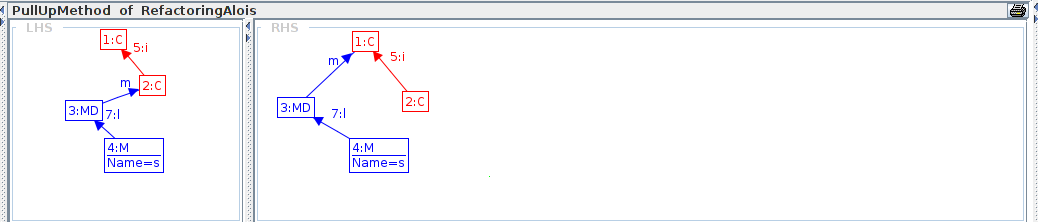
\includegraphics[width=\textwidth]{LHSRHSPullUpMethod.png}
\end{myfig}

\subsection{Précondition de refactoring}
Les préconditions servent à définir un sous graph ou un ensemble de sous graph ne pouvant pas être présent avant d'appliquer le refactoring. Nous pourrions également employé des postconditions pour interdire
certains sous graphs dans le graph résultat mais les préconditions sont plus adaptée car on évite d'appliquer des productions sur des graphs et ensuite seulement detecter une erreur.

\begin{myfig}{NACPullUpMethod}{NAC}
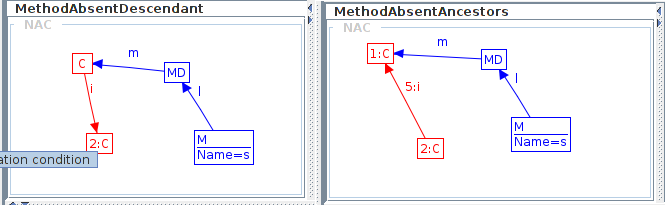
\includegraphics[width=\textwidth]{NACPullUpMethod.png}
\end{myfig}

La figure~\ref{NACPullUpMethod}, représente les deux préconditions nécessaire pour pouvoir appliquer le refactoring PullUpMethod.
Elle spécifie que aucun ancêtres ni descendants de la classe ne peut posséder cette méthode avant le refactoring.


\section{Application sur le programme transport}

\subsection{Encapsulate Variable}

Encapsuler une variable dans une classe est une opération souvent éffectué par les programmeurs. 
Elle consiste à rendre une variable public, privée et à ajouter un accesseur public et un setter public pour continuer à pouvoir accéder et à mettre à jour cette variable.

Lors d'un refactoring cela consiste à changer la visibilité de la variable et à créer deux nouvelles methodes. Ensuite il faut changer tout les accès ou/et mise à jour de la variable par des appels aux deux méthodes crées.

\subsubsection{Conditions}

\begin{itemize}[label=\textbullet]
\item Les deux nouvelles méthodes crées ne soit pas présente dans la classe
\item Les deux nouvelles méthodes crées ne soit pas présente dans ses ancêtres 
\item Les deux nouvelles méthodes crées ne soit pas présente dans ses descendants.
\end{itemize}

\subsubsection{Contraintes}

\begin{enumerate}
\item est préservée car on ne crée ni ne bougeons aucune variable.
\item est préservée car la condition stipules qu'ils ne faut pas que des méthodes comportant les même définition que le getter ou le setter soient présente.
\item est préservée car on crée deux méthodes accédant une variable dans la même classe.
\item est préservée car le paramètre de la méthodes setter est employée uniquement dans la définition de cette méthode.
\end{itemize}

\subsubsection{Avant}

\begin{lstlisting}[frame=single]
public class Person {
	public String name;
}
\end{lstlisting}

\subsubsection{Après}

\begin{lstlisting}[frame=single]
public class Person {
	private String name;
	
	public String GetName(){
		return name;
	}

	public void SetName(String n){
		name=n;
	}
}
\end{lstlisting}

\subsubsection{Représentation graphique}

\begin{myfig}{beforeEncapsulateVariable}{Before Encapsulate Variable}
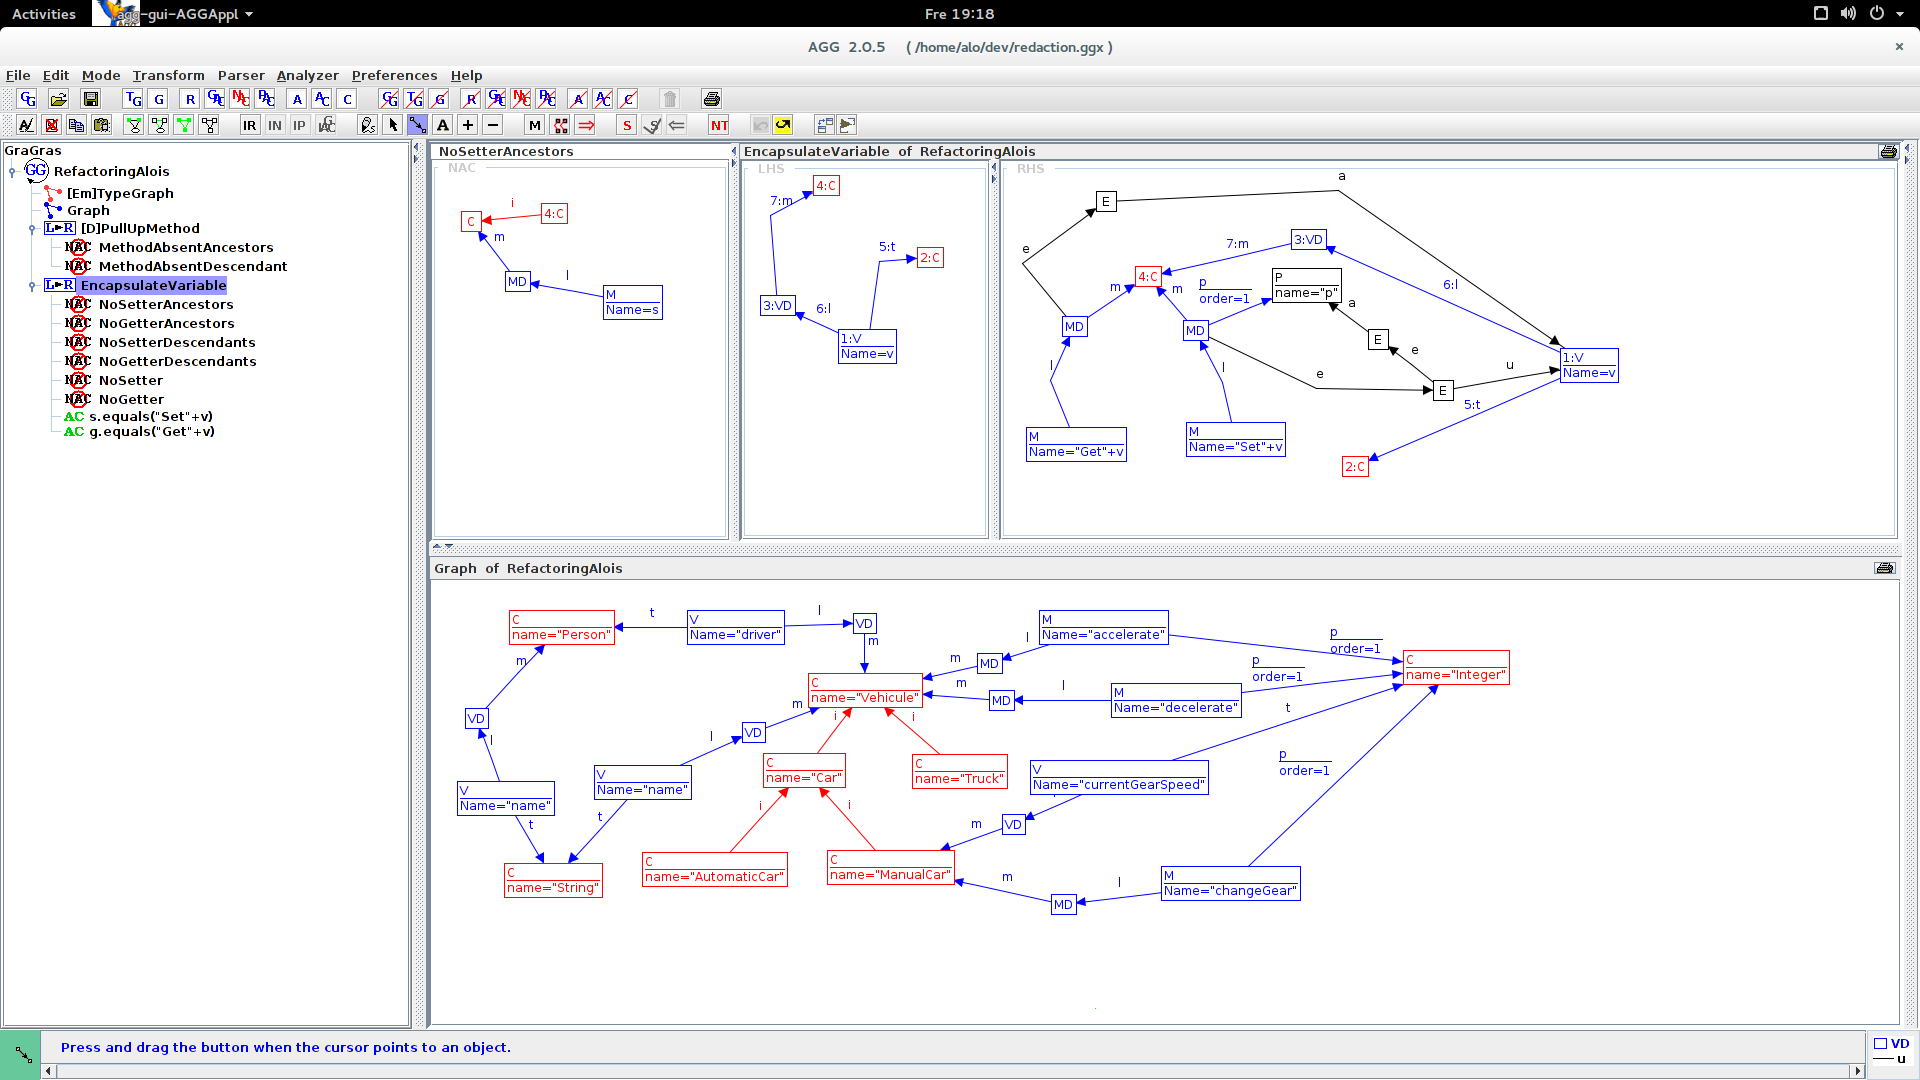
\includegraphics[width=\textwidth]{beforeEncapsulateVariable.png}
\end{myfig}

Dans le haut de la figure~\ref{beforeEncapsulateVariable} se trouve la LHS qui représente la structure d'un sous graph du programme avant sa transformation. A droite, nous avons RHS qui représente la structure de ce sous graph après la transformation. Et en dessous nous avons le graphique du programme.

\begin{myfig}{afterEncapsulateVariable}{After Encapsulate Variable}
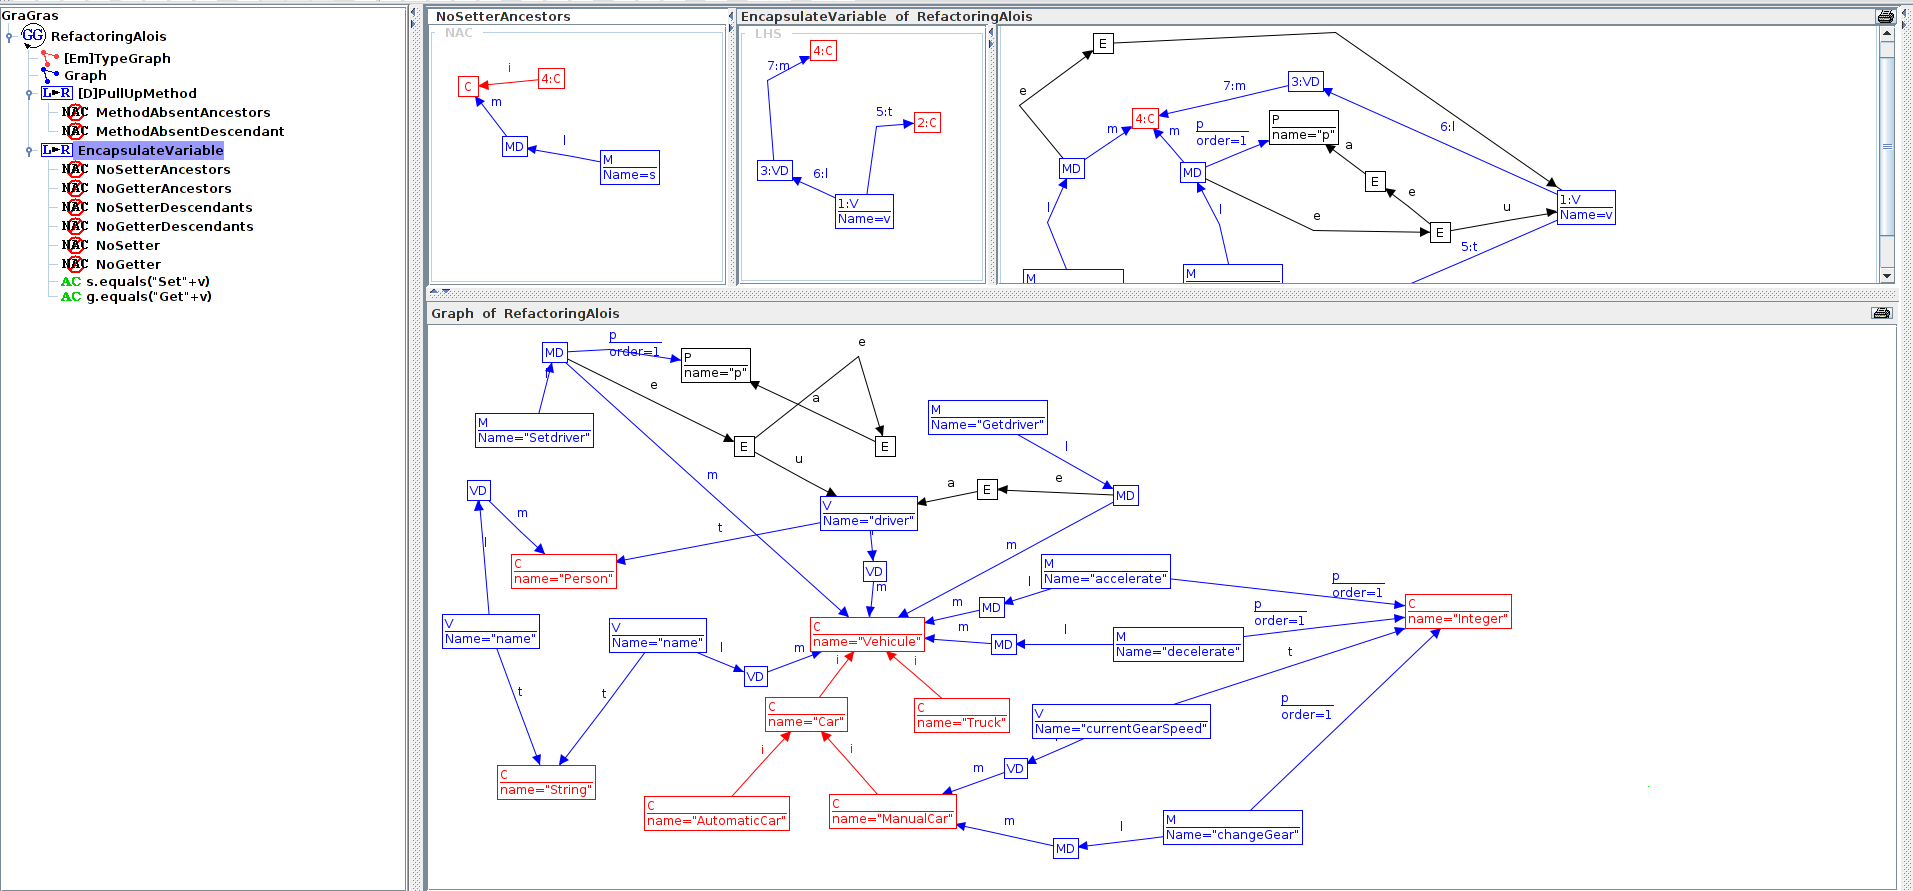
\includegraphics[width=\textwidth]{afterEncapsulateVariable.png}
\end{myfig}

Ici dans la figure~\ref{afterEncapsulateVariable} nous avons les mêmes éléments au dessus mais la partie inférieur à changer. 
Elle représente le graphique après l'application de la transformation. On peut voir que de nouveaux noeuds et de nouvelles arrêtes ont été créer pour représenter les deux nouvelles méthodes.

Je n'ai laisser que la transformation du sous graph lié à la variable "driver" pour une meilleure visibilité.

\subsection{Pull Up Method}

Cela consiste à déplacer une méthode présente dans une ou plusieur classes enfant dans la classe parent. 

\subsubsection{Conditions}

\begin{itemize}[label=\textbullet]
\item La classe parent ne peut pas déjà contenir une méthode ayant la même signature
\item Aucune des variables directement accédée ou modifiée par la méthode ne peut être en dehors du scope de la classe parent.
\end{itemize}

\subsubsection{Contraintes}

\begin{enumerate}
\item est préservée car on ne crée ni ne bougeons aucune variable.
\item est préservée grâce à la précondition qui stipule qu'il ne peut pas se trouver une méthode avec la même signature dans la classe parent.
\item est préservée grâce à la précondition qui stipule que la définition de la méthode bougée ne doit pas accéder à des variables en dehors du scope du parent.
\item est préservée car on ne crée ni ne modifie aucune méthode.
\end{enumerate}

\subsubsection{Avant}
\begin{lstlisting}[frame=single]
public class Vehicule {
	public String name;
	public Person driver;

	public void accelerating(int amount) { 
	}

	public void decelerate(int amount) { 
	}
}

public class Car extends Vehicule {

}

public class ManualCar extends Car {
	public void changeGear(int speed){ 
	}
}
\end{lstlisting}

\subsubsection{Après}
\begin{lstlisting}[frame=single]
public class Vehicule {
	public String name;
	public Person driver;

	public void accelerating(int amount) {

	}
	public void decelerate(int amount) { 
	}
	
	public void changeGear(int speed){
	}
}

public class Car extends Vehicule {

}

public class ManualCar extends Car {

}
\end{lstlisting}

\subsubsection{Représentation graphique}

\begin{myfig}{beforePullUpMethode}{Before PullUp Methode}
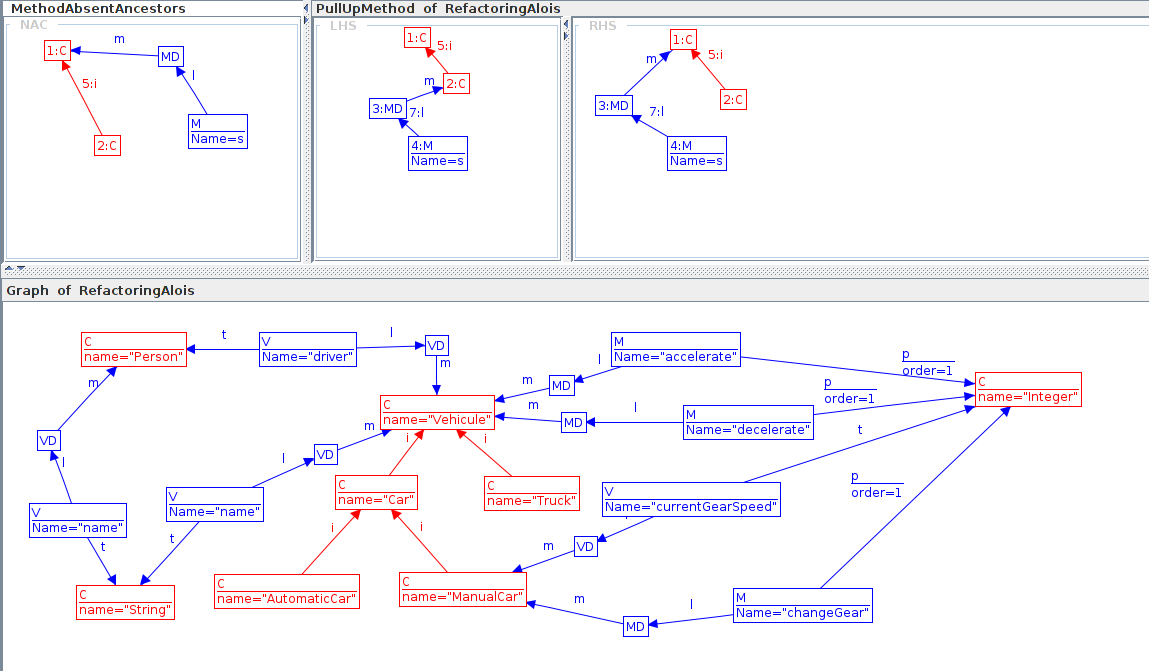
\includegraphics[width=\textwidth]{beforePullUpMethode.png}
\end{myfig}

En haut à gauche de la figure~\ref{beforePullUpMethode} se trouve la LHS qui représente la structure d'un sous graph du programme avant sa transformation. 
En haut à droite de la figure~\ref{beforePullUpMethode} se trouve la RHS qui représente la structure de ce sous graph après la transformation.
En dessous nous avons le graphique du programme.

\begin{myfig}{afterPullUpMethod}{After PullUp Methode}
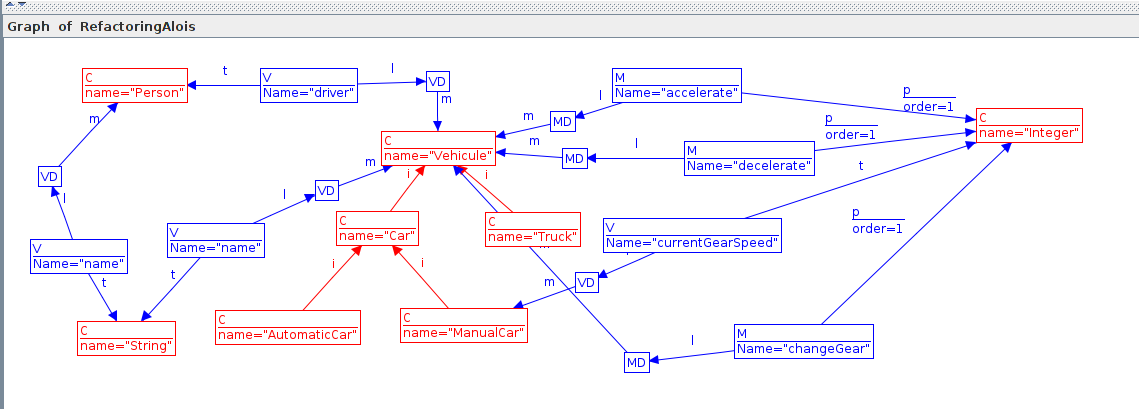
\includegraphics[width=\textwidth]{afterPullUpMethod.png}
\end{myfig}

Dans la figure~\ref{afterPullUpMethod} la partie du dessous à changé et représente le programme après avoir appliqué la transformation.
Après avoir remonté la méthode de la classe ManualCar dans la classe Vehicule, on peut observer que le lien de la méthode "changeGear" vers la classe ManualCar n'existe plus. Et qu'un nouveau lien a été créé vers la classe Vehicule.

\section{Préservation du comportement du programme}

Nous avons jusqu'ici définit des mécanismes permettent de refactorer un programme gràce aux graphs. Mais nous n'avons pas encore prouvé que ce programme conservait sont comportement à la suite de ces transformations.

Le but de cette partie est de démontrer que certaines propriétés du programme sont preservée après un refactoring:
\begin{itemize}[label=\textbullet]
\item l'accès à une variable
\item la mise à jour d'une variable
\item l'appelle d'une méthode
\end{itemize}

Pour cela nous avons besoin d'une fonction de tracking, tr.

\subsection{Définition, Préservation d'une expression de graph}
GE étant une expression de graph et G, H étant des graph de programme. La fonction tr: {$V_G$} \vec {$V_H$} est un mappage de noeuds tels que pour chaque occurence oc de GE dans G, La composition de fonction "tr \circ oc" est une occurence de GE dans H.

Pour chaque production de graph une fonction tr existe et mappe les noeuds de LHS dans ceux de RHS.

\subsection{Définition, Fonction de tracking}

\begin{myfig}{preservation}{Préservation}
MD  \mathrm{( e|c ) * u} V \mathrm{t} VD
\end{myfig}

Le graph d'expression~\ref{preservation} permet de définir que chaque définition de méthode qui met à jour une variable dans un graph de départ, doit mettre à jour cette variable dans le graph résultat.
Toutefois, cette variable peut être mis à jour par un appelle à une méthode à la place d'une mise à jour directe.



\subsection{Préservation du comportement : Encapsulate Variable}

On peut observer ici que la mise à jour de la variable dans une méthode est conservée après le refactoring, la seule différence est que l'on appéle une méthode qui met à jour la variable à la place de
directement mettre à jour la variable. Ce qui a comme résultat que le chemin de la MD jusqu'à la variable devient plus long


\section{Conclusion}

Le but de cet article était de prouver que le refactoring n'altérait pas le comportement d'un programme à l'aide de transformation de graph. En effet le code source d'un programme peut être facilement représenté avec un graph, les transformations faites à ce code source lors d'un refactoring peuvent être exprimée avec des transformations de graph et le modèle choisit est suffisant clair pour prouver que le refactoring conserve certaines propriétés du programme.

En outre certains problèmes sont apparut, ce qui a demandé des ajouts et des compromis. 

- Pour les Preconditions, certaines contraintes on été mis de coté. Par exemple pour le refactoring PullUpMethod, on ne contronlle pas que le corps de la méthode soit identique mais uniquement la signature de la méthode.

- Pour la représentation en graph, dans le but de supporté un large éventaille de language nous avons ajouté la possibilité d'attaché des attribus supplémentaires aux noeuds.

- Pour le graph de type, toutes les contraites n'étaient pas représentable à l'aide d'un graph de type, nous avons donc introduit les graph d'expression.

- Pour les transformations de graph, ?????

- Pour la préservation du comportement, ?????

Malgré ces observations, l'approche utilisée reste éfficace pour définir l'effet de chaque refactoring sur le code source d'un programme. Cependant, il est difficile à dire si cette approche formelle peut réellement servir dans une approche pratique et être employé par un outil de refactoring concret.




\end{document}
